\section{Communication routines}
%%%%%%%%%%%%%%%%%%%%%%%%%%%%%%%%%%%%%%%%%%%%%%%%%%
%
%       HALO DATA COMMUNICATION 
%
%%%%%%%%%%%%%%%%%%%%%%%%%%%%%%%%%%%%%%%%%%%%%%%%%%
The routines in this chapter implement various global communication operators
on vectors associated with a discretization mesh. For auxiliary communication
routines not tied to a discretization space see~\ref{sec:toolsrout}.

\subroutine{psb\_halo}{Halo Data Communication}    

These subroutines gathers the values of the halo
elements, and  (optionally) scale the result:

\[ x \leftarrow \alpha x \]
where:
\begin{description}
\item[$x$] is a global dense  submatrix.
\end{description}

\begin{table}[h]
\begin{center}
\begin{tabular}{ll}
\hline
$\alpha$, $x$ & {\bf Subroutine}\\
\hline
Integer           & psb\_halo \\
Short Precision Real & psb\_halo \\
Long Precision Real & psb\_halo \\
Short Precision Complex & psb\_halo \\
Long Precision Complex & psb\_halo \\
\hline
\end{tabular}
\end{center}
\caption{Data types\label{tab:f90halo}}
\end{table}

\syntax{call psb\_halo}{x, desc\_a, info}
\syntax*{call psb\_halo}{x, desc\_a, info, alpha, work, data}

\begin{description}
\item[Type:] Synchronous.
\item[\bf On Entry]
\item[x] global dense matrix $x$.\\
Scope: {\bf local} \\
Type: {\bf required} \\
Intent: {\bf inout}.\\
Specified as:  a rank one or two array with the TARGET attribute
containing numbers of type specified in
Table~\ref{tab:f90halo}.
\item[desc\_a] contains data structures for communications.\\
Scope: {\bf local} \\
Type: {\bf required}\\
Intent: {\bf in}.\\
Specified as: a structured data of type \descdata.
\item[alpha] the scalar $\alpha$.\\
Scope: {\bf global} \\
Type: {\bf optional} \\
Intent: {\bf in}.\\
Default: $alpha = 1 $\\	
Specified as: a number of the data type indicated in Table~\ref{tab:f90halo}.
\item[work] the work array. \\
Scope: {\bf local} \\
Type: {\bf optional}\\
Intent: {\bf inout}.\\
Specified as: a rank one array of the same type of $x$ with the
POINTER attribute.
\item[data] index list selector.\\
Scope: {\bf global} \\
Type: {\bf optional} \\
Specified as: an integer. Values:\verb|psb_comm_halo_|,\verb|psb_comm_mov_|,
\verb|psb_comm_ext_|, default: \verb|psb_comm_halo_|. Chooses the
index list on which to base the data exchange. 


\item[\bf On Return] 
\item[x] global dense result matrix $x$.\\
Scope: {\bf local} \\
Type: {\bf required} \\
Intent: {\bf inout}.\\
Returned as:  a rank one or two array 
containing numbers of type specified in
Table~\ref{tab:f90halo}.
\item[info] the local portion of result submatrix $y$.\\
Scope: {\bf local} \\
Type: {\bf required} \\
Intent: {\bf out}.\\
An integer value that contains an error code. 
\end{description}
\begin{figure}[h] \begin{center}
\rotatebox{-90}{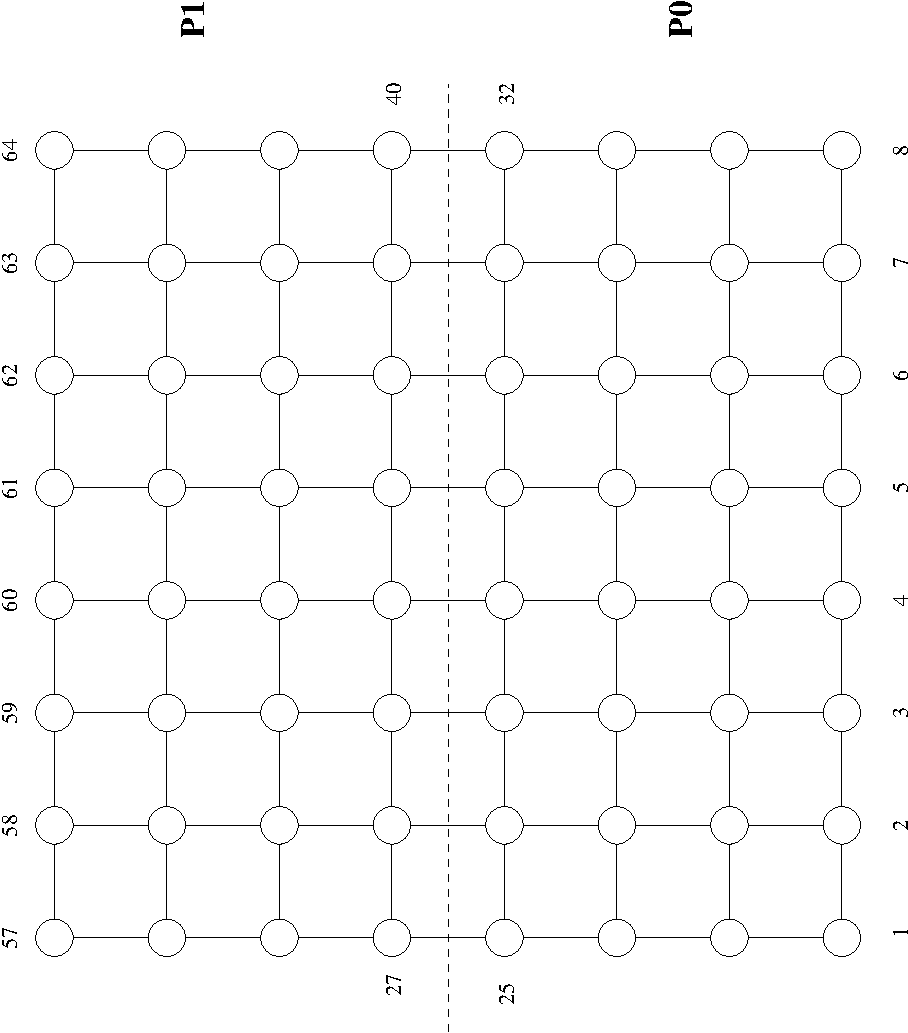
\includegraphics[scale=0.45]{figures/try8x8}}
\end{center}
\caption{Sample discretization mesh.\label{fig:try8x8}}
\end{figure}
\section*{Example of use}
Consider the discretization mesh depicted in fig.~\ref{fig:try8x8},
partitioned among two processes as shown by the dashed line; the data
distribution is such that each process will own 32 entries in the
index space, with a halo made of 8 entries placed at local indices 33
through 40. If process 0 assigns an initial value of 1 to its entries
in the $x$ vector, and process 1 assigns a value of 2, then after a
call to \verb|psb_halo| the contents of the local vectors will be the
following: 
\begin{table}
\begin{center}
\small\begin{tabular}{rrr@{\hspace{6\tabcolsep}}rrr}
\multicolumn{3}{c}{Process  0}&
\multicolumn{3}{c}{Process  1}\\
  I  &   GLOB(I) & X(I)  &   I & GLOB(I) & X(I) \\
  1   &    1  &  1.0   &   1  &  33  &   2.0 \\ 
  2   &    2  &  1.0   &   2  &  34  &   2.0 \\
  3   &    3  &  1.0   &   3  &  35  &   2.0 \\
  4   &    4  &  1.0   &   4  &  36  &   2.0 \\
  5   &    5  &  1.0   &   5  &  37  &   2.0 \\
  6   &    6  &  1.0   &   6  &  38  &   2.0 \\
  7   &    7  &  1.0   &   7  &  39  &   2.0 \\
  8   &    8  &  1.0   &   8  &  40  &   2.0 \\
  9   &    9  &  1.0   &   9  &  41  &   2.0 \\
 10   &   10  &  1.0   &  10  &  42  &   2.0 \\
 11   &   11  &  1.0   &  11  &  43  &   2.0 \\
 12   &   12  &  1.0   &  12  &  44  &   2.0 \\
 13   &   13  &  1.0   &  13  &  45  &   2.0 \\
 14   &   14  &  1.0   &  14  &  46  &   2.0 \\
 15   &   15  &  1.0   &  15  &  47  &   2.0 \\
 16   &   16  &  1.0   &  16  &  48  &   2.0 \\
 17   &   17  &  1.0   &  17  &  49  &   2.0 \\
 18   &   18  &  1.0   &  18  &  50  &   2.0 \\
 19   &   19  &  1.0   &  19  &  51  &   2.0 \\
 20   &   20  &  1.0   &  20  &  52  &   2.0 \\ 
21   &   21  &  1.0   &  21  &  53  &   2.0 \\
22   &   22  &  1.0   &  22  &  54  &   2.0 \\
23   &   23  &  1.0   &  23  &  55  &   2.0 \\
24   &   24  &  1.0   &  24  &  56  &   2.0 \\
25   &   25  &  1.0   &  25  &  57  &   2.0 \\
26   &   26  &  1.0   &  26  &  58  &   2.0 \\
27   &   27  &  1.0   &  27  &  59  &   2.0 \\
28   &   28  &  1.0   &  28  &  60  &   2.0 \\
29   &   29  &  1.0   &  29  &  61  &   2.0 \\
30   &   30  &  1.0   &  30  &  62  &   2.0 \\
31   &   31  &  1.0   &  31  &  63  &   2.0 \\
32   &   32  &  1.0   &  32  &  64  &   2.0 \\
33   &   33  &  2.0   &  33  &  25  &   1.0 \\
34   &   34  &  2.0   &  34  &  26  &   1.0 \\
35   &   35  &  2.0   &  35  &  27  &   1.0 \\
36   &   36  &  2.0   &  36  &  28  &   1.0 \\
37   &   37  &  2.0   &  37  &  29  &   1.0 \\
38   &   38  &  2.0   &  38  &  30  &   1.0 \\
39   &   39  &  2.0   &  39  &  31  &   1.0 \\
40   &   40  &  2.0   &  40  &  32  &   1.0 \\
\end{tabular}
\end{center}
\end{table}

%%%%%%%%%%%%%%%%%%%%%%%%%%%%%%%%%%%%%%%%%%%%%%%%%%
%
%       OVERLAP UPDATE
%
%%%%%%%%%%%%%%%%%%%%%%%%%%%%%%%%%%%%%%%%%%%%%%%%%%


\subroutine{psb\_ovrl}{Overlap Update}    

These subroutines applies an overlap operator to the input vector:

\[ x \leftarrow Q x \]
where:
\begin{description}
\item[$x$] is the global dense submatrix $x$
\item[$Q$] is the overlap operator; it is the composition of two
operators $ P_a$ and $ P^{T}$. 
\end{description}

\begin{table}[h]
\begin{center}
\begin{tabular}{ll}
\hline
$x$ & {\bf Subroutine}\\
\hline
Short Precision Real & psb\_ovrl \\
Long Precision Real & psb\_ovrl \\
Short Precision Complex & psb\_ovrl \\
Long Precision Complex & psb\_ovrl \\
\hline
\end{tabular}
\end{center}
\caption{Data types\label{tab:f90ovrl}}
\end{table}

\syntax{call psb\_ovrl}{x, desc\_a, info}
\syntax*{call psb\_ovrl}{x, desc\_a, info, update=update\_type, work=work} 

\begin{description}
\item[Type:] Synchronous.
\item[\bf On Entry]
\item[x] global dense matrix $x$.\\
Scope: {\bf local} \\
Type: {\bf required} \\
Intent: {\bf inout}.\\
Specified as:  a rank one or two array 
containing numbers of type specified in
Table~\ref{tab:f90ovrl}.
\item[desc\_a] contains data structures for communications.\\
Scope: {\bf local} \\
Type: {\bf required}\\
Intent: {\bf in}.\\
Specified as: a structured data of type \descdata.
\item[update] Update operator. \\
\begin{description}
\item[update = psb\_none\_] Do nothing;
\item[update = psb\_add\_] Sum overlap entries, i.e. apply $P^T$;
\item[update = psb\_avg\_] Average overlap entries, i.e. apply $P_aP^T$;
%% \item[update = psb\_square\_root\_] square root update $\sqrt{P_a}$;
\end{description}
Scope: {\bf global} \\
Intent: {\bf in}.\\
Default: $update\_type = psb\_avg\_ $\\	
Scope: {\bf global} \\
Specified as: a integer variable.
\item[work] the work array. \\
Scope: {\bf local} \\
Type: {\bf optional}\\
Intent: {\bf inout}.\\
Specified as: a one dimensional array of the same type of $x$.

\item[\bf On Return] 
\item[x] global dense result matrix $x$.\\
Scope: {\bf local} \\
Type: {\bf required} \\
Intent: {\bf inout}.\\
Specified as: an  array of rank one or two
containing numbers of type specified in
Table~\ref{tab:f90ovrl}.
\item[info] Error code.\\
Scope: {\bf local} \\
Type: {\bf required} \\
Intent: {\bf out}.\\
An integer value; 0 means no error has been detected. 
\end{description}


\section*{Usage notes}
\begin{enumerate}
\item If there is no overlap in the data distribution associated with
  the descriptor, no operations are performed;
\item The operator $P^{T}$ performs the reduction sum of overlap
elements; it is a ``prolongation'' operator $P^T$ that
replicates overlap elements, accounting for the physical replication
of data;
\item The operator $P_a$ performs a scaling on the overlap elements by
the amount of replication; thus, when combined with the reduction
operator, it implements the average of replicated elements over all of
their instances. 
%% \item The square root update option makes it possible to applythe
%% following operator: 
%% \[ x\leftarrow \sqrt{P_a} P^{T} K^{-1} P \sqrt{P_a} x\]
%% In the case of a symmetric $K$, this preserves simmetry of the overall
%% preconditioner, which would otherwise be destroyed. 
\end{enumerate}
 
\begin{figure}[h] \begin{center}
\rotatebox{-90}{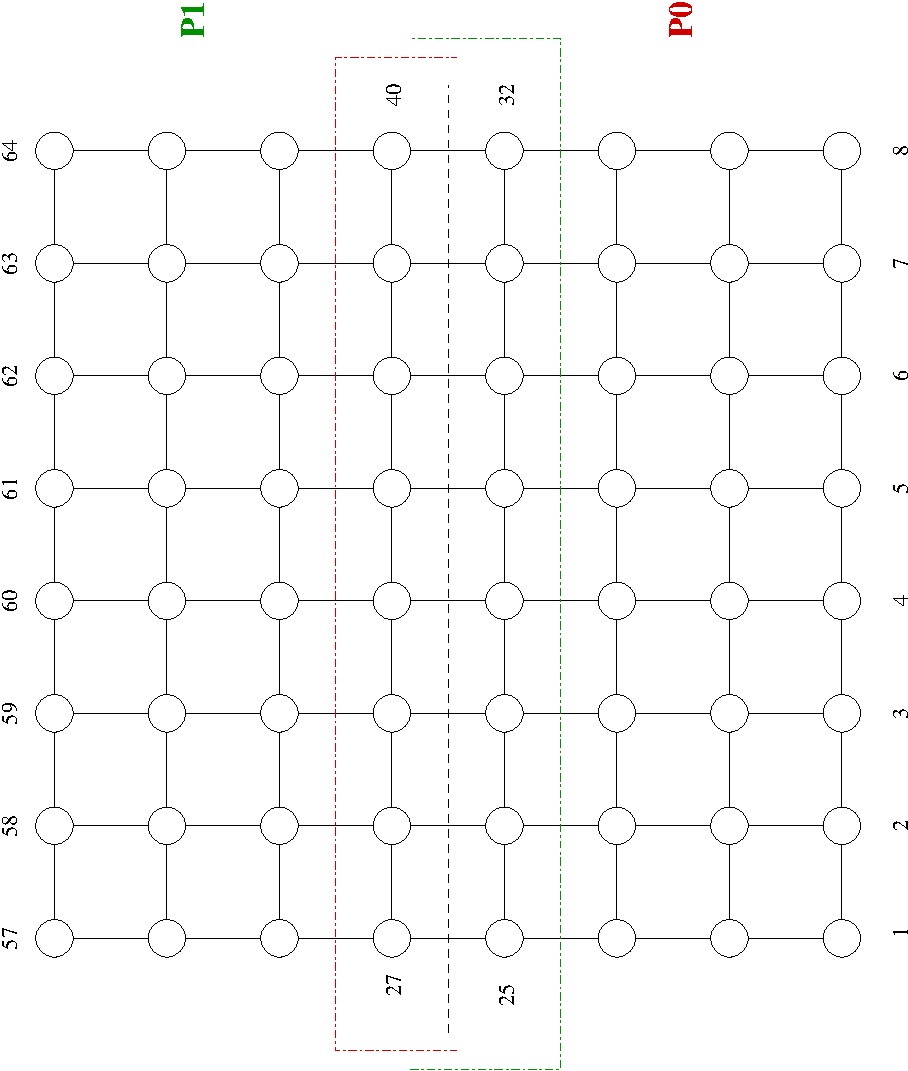
\includegraphics[scale=0.65]{figures/try8x8_ov}}
\end{center}
\caption{Sample discretization mesh.\label{fig:try8x8_ov}}
\end{figure}
\section*{Example of use}
Consider the discretization mesh depicted in fig.~\ref{fig:try8x8_ov},
partitioned among two processes as shown by the dashed lines, with an
overlap of 1 extra layer with respect to the partition of
fig.~\ref{fig:try8x8}; the data 
distribution is such that each process will own 40 entries in the
index space, with an overlap of 16  entries placed at local indices 25 
through 40; the halo will run from local index 41 through local index 48.. If process 0 assigns an initial value of 1 to its entries
in the $x$ vector, and process 1 assigns a value of 2, then after a
call to \verb|psb_ovrl| with \verb|psb_avg_| and a call to
\verb|psb_halo_| the contents of the local vectors will be the
following (showing a transition among the two subdomains)  

\begin{table}
\begin{center}
\footnotesize
\begin{tabular}{rrr@{\hspace{6\tabcolsep}}rrr}
\multicolumn{3}{c}{Process  0}&
\multicolumn{3}{c}{Process  1}\\
  I  &   GLOB(I) & X(I)  &   I & GLOB(I) & X(I) \\
  1   &    1  &  1.0   &   1  &  33  &   1.5 \\ 
  2   &    2  &  1.0   &   2  &  34  &   1.5 \\
  3   &    3  &  1.0   &   3  &  35  &   1.5 \\
  4   &    4  &  1.0   &   4  &  36  &   1.5 \\
  5   &    5  &  1.0   &   5  &  37  &   1.5 \\
  6   &    6  &  1.0   &   6  &  38  &   1.5 \\
  7   &    7  &  1.0   &   7  &  39  &   1.5 \\
  8   &    8  &  1.0   &   8  &  40  &   1.5 \\
  9   &    9  &  1.0   &   9  &  41  &   2.0 \\
 10   &   10  &  1.0   &  10  &  42  &   2.0 \\
 11   &   11  &  1.0   &  11  &  43  &   2.0 \\
 12   &   12  &  1.0   &  12  &  44  &   2.0 \\
 13   &   13  &  1.0   &  13  &  45  &   2.0 \\
 14   &   14  &  1.0   &  14  &  46  &   2.0 \\
 15   &   15  &  1.0   &  15  &  47  &   2.0 \\
 16   &   16  &  1.0   &  16  &  48  &   2.0 \\
 17   &   17  &  1.0   &  17  &  49  &   2.0 \\
 18   &   18  &  1.0   &  18  &  50  &   2.0 \\
 19   &   19  &  1.0   &  19  &  51  &   2.0 \\
 20   &   20  &  1.0   &  20  &  52  &   2.0 \\ 
 21   &   21  &  1.0   &  21  &  53  &   2.0 \\
 22   &   22  &  1.0   &  22  &  54  &   2.0 \\
 23   &   23  &  1.0   &  23  &  55  &   2.0 \\
 24   &   24  &  1.0   &  24  &  56  &   2.0 \\
 25   &   25  &  1.5   &  25  &  57  &   2.0 \\
 26   &   26  &  1.5   &  26  &  58  &   2.0 \\
 27   &   27  &  1.5   &  27  &  59  &   2.0 \\
 28   &   28  &  1.5   &  28  &  60  &   2.0 \\
 29   &   29  &  1.5   &  29  &  61  &   2.0 \\
 30   &   30  &  1.5   &  30  &  62  &   2.0 \\
 31   &   31  &  1.5   &  31  &  63  &   2.0 \\
 32   &   32  &  1.5   &  32  &  64  &   2.0 \\
 33   &   33  &  1.5   &  33  &  25  &   1.5 \\
 34   &   34  &  1.5   &  34  &  26  &   1.5 \\
 35   &   35  &  1.5   &  35  &  27  &   1.5 \\
 36   &   36  &  1.5   &  36  &  28  &   1.5 \\
 37   &   37  &  1.5   &  37  &  29  &   1.5 \\
 38   &   38  &  1.5   &  38  &  30  &   1.5 \\
 39   &   39  &  1.5   &  39  &  31  &   1.5 \\
 40   &   40  &  1.5   &  40  &  32  &   1.5 \\
 41   &   41  &  2.0   &  41  &  17  &   1.0 \\
 42   &   42  &  2.0   &  42  &  18  &   1.0 \\
 43   &   43  &  2.0   &  43  &  19  &   1.0 \\
 44   &   44  &  2.0   &  44  &  20  &   1.0 \\
 45   &   45  &  2.0   &  45  &  21  &   1.0 \\
 46   &   46  &  2.0   &  46  &  22  &   1.0 \\
 47   &   47  &  2.0   &  47  &  23  &   1.0 \\
 48   &   48  &  2.0   &  48  &  24  &   1.0 \\
\end{tabular}
\end{center}
\end{table}



%%%%%%%%%%%%%%%%%%%%%%%%%%%%%%%%%%%%%%%%%%%%%%%%%%
%
%      GATHER GLOBAL DENSE MATRIX
%
%%%%%%%%%%%%%%%%%%%%%%%%%%%%%%%%%%%%%%%%%%%%%%%%%%

\subroutine{psb\_gather}{Gather Global Dense Matrix}

These subroutines collect the portions of global dense matrix
distributed over all process into one single array stored on one
process.

\[ glob\_x \leftarrow collect(loc\_x_i) \]
where:
\begin{description}
\item[$glob\_x$] is the global submatrix $glob\_x_{1:m,1:n}$
\item[$loc\_x_i$] is the local portion of global dense matrix on
process $i$.
\item[$collect$] is the collect function.
\end{description}

\begin{table}[h]
\begin{center}
\begin{tabular}{ll}
\hline
$x_i, y$ & {\bf Subroutine}\\
\hline
Integer            & psb\_gather \\
Short Precision Real & psb\_gather \\
Long Precision Real & psb\_gather \\
Short Precision Complex & psb\_gather \\
Long Precision Complex & psb\_gather \\
\hline
\end{tabular}
\end{center}
\caption{Data types\label{tab:gather}}
\end{table}

\syntax{call psb\_gather}{glob\_x, loc\_x, desc\_a, info, root}
\syntax{call psb\_gather}{glob\_x, loc\_x, desc\_a, info, root}

\begin{description}
\item[Type:] Synchronous.
\item[\bf On Entry]
\item[loc\_x] the local portion of global dense matrix
$glob\_x$. \\
Scope: {\bf local} \\
Type: {\bf required}\\
Intent: {\bf in}.\\
Specified as: a rank one or two array containing numbers of the type
indicated in Table~\ref{tab:gather}.
\item[desc\_a] contains data structures for communications.\\
Scope: {\bf local} \\
Type: {\bf required}\\
Intent: {\bf in}.\\
Specified as: a structured data of type \descdata.
\item[root]  The process that holds the global copy. If $root=-1$ all
  the processes will have a copy of the global vector.\\
Scope: {\bf global} \\
Type: {\bf optional}\\
Intent: {\bf in}.\\
Specified as: an integer variable $-1\le root\le np-1$, default $-1$. 
%% \item[iglobx]  Row index to define a submatrix in glob\_x into which
%%   gather the local pieces.\\
%% Scope: {\bf global} \\
%% Type: {\bf optional}\\
%% Specified as: an integer variable $1\le ix\le matrix\_data(psb\_m\_)$. 
%% \item[jglobx]  Column index to define a submatrix in glob\_x into which
%%   gather the local pieces.\\
%% Scope: {\bf global} \\
%% Type: {\bf optional}\\
%% Specified as: an integer variable. 
%% \item[ilocx]  Row index to define a submatrix in loc\_x that has to
%%   be gathered into glob\_x.\\
%% Scope: {\bf local} \\
%% Type: {\bf optional}\\
%% Specified as: an integer variable. 
%% \item[jlocx]  Columns index to define a submatrix in loc\_x that has
%%   to be gathered into glob\_x.\\
%% Scope: {\bf global} \\
%% Type: {\bf optional}\\
%% Specified as: an integer variable.
%% \item[k]  The number of columns to gather.\\
%% Scope: {\bf global} \\
%% Type: {\bf optional}\\
%% Specified as: an integer variable. 
\item[\bf On Return] 
\item[glob\_x] The array where the local parts must be gathered.\\
Scope: {\bf global} \\
Type: {\bf required}\\
Intent: {\bf out}.\\
Specified as: a rank one or two array.
\item[info] Error code.\\
Scope: {\bf local} \\
Type: {\bf required} \\
Intent: {\bf out}.\\
An integer value; 0 means no error has been detected. 
\end{description}

%%%%%%%%%%%%%%%%%%%%%%%%%%%%%%%%%%%%%%%%%%%%%%%%%%
%
%      SCATTER GLOBAL DENSE MATRIX
%
%%%%%%%%%%%%%%%%%%%%%%%%%%%%%%%%%%%%%%%%%%%%%%%%%%

\subroutine{psb\_scatter}{Scatter Global Dense Matrix}

These subroutines scatters the portions of global dense matrix owned
by a process to all the processes in the processes grid.

\[ loc\_x_i \leftarrow scatter(glob\_x) \]
where:
\begin{description}
\item[$glob\_x$] is the global matrix $glob\_x_{1:m,1:n}$
\item[$loc\_x_i$] is the local portion of global dense matrix on
process $i$.
\item[$scatter$] is the scatter function.
\end{description}

\begin{table}[h]
\begin{center}
\begin{tabular}{ll}
\hline
$x_i, y$ & {\bf Subroutine}\\
\hline
Integer          & psb\_scatter \\
Short Precision Real & psb\_scatter \\
Long Precision Real & psb\_scatter \\
Short Precision Complex & psb\_scatter \\
Long Precision Complex & psb\_scatter \\
\hline
\end{tabular}
\end{center}
\caption{Data types\label{tab:scatter}}
\end{table}

\syntax{call psb\_scatter}{glob\_x, loc\_x, desc\_a, info, root}
\syntax{call psb\_scatter}{glob\_x, loc\_x, desc\_a, info, root}

\begin{description}
\item[Type:] Synchronous.
\item[\bf On Entry]
\item[glob\_x] The array that must be scattered into local pieces.\\
Scope: {\bf global} \\
Type: {\bf required}\\
Intent: {\bf in}.\\
Specified as: a rank one or two array.
\item[desc\_a] contains data structures for communications.\\
Scope: {\bf local} \\
Type: {\bf required}\\
Intent: {\bf in}.\\
Specified as: a structured data of type \descdata.
\item[root]  The process that holds the global copy. If $root=-1$ all
  the processes have a copy of the global vector.\\
Scope: {\bf global} \\
Type: {\bf optional}\\
Intent: {\bf in}.\\
Specified as: an integer variable $-1\le root\le np-1$, default $-1$. 
%% \item[iglobx]  Row index to define a submatrix in glob\_x that has to
%%   be scattered into local pieces.\\
%% Scope: {\bf global} \\
%% Type: {\bf optional}\\
%% Specified as: an integer variable $1\le ix\le matrix\_data(psb\_m\_)$. 
%% \item[jglobx]  Column index to define a submatrix in glob\_x that has to
%%   be scattered into local pieces.\\
%% Scope: {\bf global} \\
%% Type: {\bf optional}\\
%% Specified as: an integer variable. 
%% \item[ilocx]  Row index to define a submatrix in loc\_x into which
%%   scatter the local piece of glob\_x.\\
%% Scope: {\bf local} \\
%% Type: {\bf optional}\\
%% Specified as: an integer variable. 
%% \item[jlocx]  Columns index to define a submatrix in loc\_x into which
%%   scatter the local piece of glob\_x.\\
%% Scope: {\bf global} \\
%% Type: {\bf optional}\\
%% Specified as: an integer variable.
%% \item[k]  The number of columns to scatter.\\
%% Scope: {\bf global} \\
%% Type: {\bf optional}\\
%% Specified as: an integer variable. 
\item[\bf On Return] 
\item[loc\_x] the local portion of global dense matrix
$glob\_x$. \\
Scope: {\bf local} \\
Type: {\bf required}\\
Intent: {\bf out}.\\
Specified as: a rank one or two array containing numbers of the type
indicated in Table~\ref{tab:scatter}.
\item[info] Error code.\\
Scope: {\bf local} \\
Type: {\bf required} \\
Intent: {\bf out}.\\
An integer value; 0 means no error has been detected. 
\end{description}

%%% Local Variables: 
%%% mode: latex
%%% TeX-master: "userguide"
%%% End: 
